\documentclass[a4paper,12pt]{article} 

% First, we usually want to set the margins of our document. For this we use the package geometry.
\usepackage[top = 2.5cm, bottom = 2.5cm, left = 2.5cm, right = 2.5cm]{geometry} 
\usepackage[T1]{fontenc}
\usepackage[utf8]{inputenc}

% The following two packages - multirow and booktabs - are needed to create nice looking tables.
\usepackage{multirow} % Multirow is for tables with multiple rows within one cell.
\usepackage{booktabs} % For even nicer tables.

% As we usually want to include some plots (.pdf files) we need a package for that.
\usepackage{graphicx} 

% The default setting of LaTeX is to indent new paragraphs. This is useful for articles. But not really nice for homework problem sets. The following command sets the indent to 0.
%\usepackage{setspace}
%\setlength{\parindent}{0in}
\usepackage{indentfirst}

% Package to place figures where you want them.
\usepackage{float}

% The fancyhdr package let's us create nice headers.
\usepackage{fancyhdr}

\usepackage{amsmath,amsthm,caption,tikz}

% To make our document nice we want a header and number the pages in the footer.

\pagestyle{fancy} % With this command we can customize the header style.

\fancyhf{} % This makes sure we do not have other information in our header or footer.

\lhead{\footnotesize Data Structure and Algorithm Analysis(H): Work Sheet 8}% \lhead puts text in the top left corner. \footnotesize sets our font to a smaller size.

%\rhead works just like \lhead (you can also use \chead)
\rhead{\footnotesize Mengxuan Wu} %<---- Fill in your lastnames.

% Similar commands work for the footer (\lfoot, \cfoot and \rfoot).
% We want to put our page number in the center.
\cfoot{\footnotesize \thepage} 

\begin{document}

\thispagestyle{empty} % This command disables the header on the first page. 

\begin{tabular}{p{15.5cm}}
{\large \bf Data Structure and Algorithm Analysis(H)} \\
Southern University of Science and Technology \\ Mengxuan Wu \\ 12212006 \\
\hline
\\
\end{tabular}

\vspace*{0.3cm} %add some vertical space in between the line and our title.

\begin{center}
	{\Large \bf Work Sheet 8}
	\vspace{2mm}

	{\bf Mengxuan Wu}
		
\end{center}  

\vspace{0.4cm}

\section*{Question 8.1}

\subsection*{1.}

\begin{figure}[H]
	\begin{minipage}{0.133\linewidth}
		\centering
		\begin{tabular}{|c|}
			\hline
			\\ \hline
			\\ \hline
			7 \\ \hline
		\end{tabular}
		\caption*{\textsc{Push}$(S,7)$}
	\end{minipage}
	\begin{minipage}{0.133\linewidth}
		\centering
		\begin{tabular}{|c|}
			\hline
			\\ \hline
			4 \\ \hline
			7 \\ \hline
		\end{tabular}
		\caption*{\textsc{Push}$(S,4)$}
	\end{minipage}
	\begin{minipage}{0.133\linewidth}
		\centering
		\begin{tabular}{|c|}
			\hline
			5 \\ \hline
			4 \\ \hline
			7 \\ \hline
		\end{tabular}
		\caption*{\textsc{Push}$(S,5)$}
	\end{minipage}
	\begin{minipage}{0.133\linewidth}
		\centering
		\begin{tabular}{|c|}
			\hline
			\\ \hline
			4 \\ \hline
			7 \\ \hline
		\end{tabular}
		\caption*{\textsc{Pop}$(S)$}
	\end{minipage}
	\begin{minipage}{0.133\linewidth}
		\centering
		\begin{tabular}{|c|}
			\hline
			8 \\ \hline
			4 \\ \hline
			7 \\ \hline
		\end{tabular}
		\caption*{\textsc{Push}$(S,8)$}
	\end{minipage}
	\begin{minipage}{0.133\linewidth}
		\centering
		\begin{tabular}{|c|}
			\hline
			\\ \hline
			4 \\ \hline
			7 \\ \hline
		\end{tabular}
		\caption*{\textsc{Pop}$(S)$}
	\end{minipage}
	\begin{minipage}{0.133\linewidth}
		\centering
		\begin{tabular}{|c|}
			\hline
			\\ \hline
			\\ \hline
			7 \\ \hline
		\end{tabular}
		\caption*{\textsc{Pop}$(S)$}
	\end{minipage}
\end{figure}

\subsection*{2.}

\begin{center}
	\begin{tabular}{|c|c|c|c|c|}
		\hline
		7 & & & & \textsc{Enqueue}$(Q,7)$ \\ \hline \hline
		7 & 4 & & & \textsc{Enqueue}$(Q,4)$ \\ \hline \hline
		7 & 4 & 5 & & \textsc{Enqueue}$(Q,5)$ \\ \hline \hline
		& 4 & 5 & & \textsc{Dequeue}$(Q)$ \\ \hline \hline
		& 4 & 5 & 8 & \textsc{Enqueue}$(Q,8)$ \\ \hline \hline
		& & 5 & 8 & \textsc{Dequeue}$(Q)$ \\ \hline \hline
		& & & 8 & \textsc{Dequeue}$(Q)$ \\ \hline
	\end{tabular}
\end{center}

\subsection*{3.}

\begin{figure}[H]
	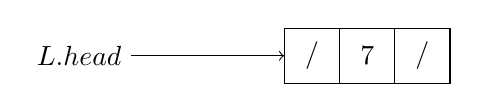
\begin{tikzpicture}
		\draw (3,0) node[minimum size = 0.7cm, draw] (mid1) {7};
		\draw (3.7,0) node[minimum size = 0.7cm, draw] (tail1) {/};
		\draw (2.3,0) node[minimum size = 0.7cm, draw] (head1) {/};

		\draw (0,0) node [left] (Lhead) {$L.head$};
		\draw [->] (Lhead) -- (head1.west);
	\end{tikzpicture}
	\caption*{\textsc{List-Prepend}$(L,7)$}
\end{figure}

\begin{figure}[H]
	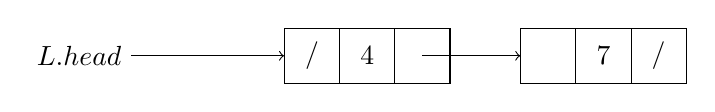
\begin{tikzpicture}
		\draw (3,0) node[minimum size = 0.7cm, draw] (mid1) {4};
		\draw (3.7,0) node[minimum size = 0.7cm, draw] (tail1) {};
		\draw (2.3,0) node[minimum size = 0.7cm, draw] (head1) {/};

		\draw (6,0) node[minimum size = 0.7cm, draw] (mid2) {7};
		\draw (6.7,0) node[minimum size = 0.7cm, draw] (tail2) {/};
		\draw (5.3,0) node[minimum size = 0.7cm, draw] (head2) {};

		\draw (0,0) node [left] (Lhead) {$L.head$};

		\draw [->] (Lhead) -- (head1.west);
		\draw [->] (tail1.center) -- (head2.west);
	\end{tikzpicture}
	\caption*{\textsc{List-Prepend}$(L,4)$}
\end{figure}

\begin{figure}[H]
	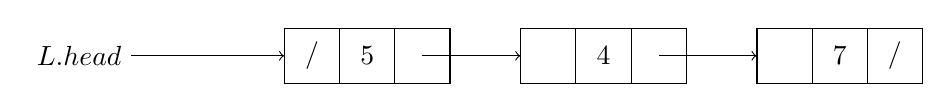
\begin{tikzpicture}
		\draw (3,0) node[minimum size = 0.7cm, draw] (mid1) {5};
		\draw (3.7,0) node[minimum size = 0.7cm, draw] (tail1) {};
		\draw (2.3,0) node[minimum size = 0.7cm, draw] (head1) {/};

		\draw (6,0) node[minimum size = 0.7cm, draw] (mid2) {4};
		\draw (6.7,0) node[minimum size = 0.7cm, draw] (tail2) {};
		\draw (5.3,0) node[minimum size = 0.7cm, draw] (head2) {};

		\draw (9,0) node[minimum size = 0.7cm, draw] (mid3) {7};
		\draw (9.7,0) node[minimum size = 0.7cm, draw] (tail3) {/};
		\draw (8.3,0) node[minimum size = 0.7cm, draw] (head3) {};

		\draw (0,0) node [left] (Lhead) {$L.head$};

		\draw [->] (Lhead) -- (head1.west);
		\draw [->] (tail1.center) -- (head2.west);
		\draw [->] (tail2.center) -- (head3.west);
	\end{tikzpicture}
	\caption*{\textsc{List-Prepend}$(L,5)$}
\end{figure}

\begin{figure}[H]
	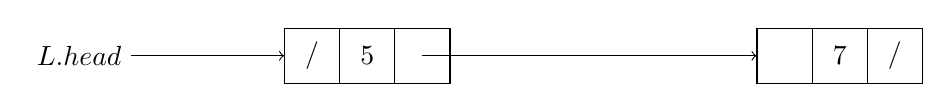
\begin{tikzpicture}
		\draw (3,0) node[minimum size = 0.7cm, draw] (mid1) {5};
		\draw (3.7,0) node[minimum size = 0.7cm, draw] (tail1) {};
		\draw (2.3,0) node[minimum size = 0.7cm, draw] (head1) {/};

		\draw (9,0) node[minimum size = 0.7cm, draw] (mid3) {7};
		\draw (9.7,0) node[minimum size = 0.7cm, draw] (tail3) {/};
		\draw (8.3,0) node[minimum size = 0.7cm, draw] (head3) {};

		\draw (0,0) node [left] (Lhead) {$L.head$};

		\draw [->] (Lhead) -- (head1.west);
		\draw [->] (tail1.center) -- (head3.west);
	\end{tikzpicture}
	\caption*{\textsc{List-Delete}$(L,4)$}
\end{figure}

\begin{figure}[H]
	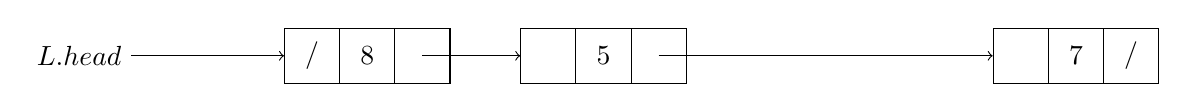
\begin{tikzpicture}
		\draw (3,0) node[minimum size = 0.7cm, draw] (mid4) {8};
		\draw (3.7,0) node[minimum size = 0.7cm, draw] (tail4) {};
		\draw (2.3,0) node[minimum size = 0.7cm, draw] (head4) {/};

		\draw (6,0) node[minimum size = 0.7cm, draw] (mid1) {5};
		\draw (6.7,0) node[minimum size = 0.7cm, draw] (tail1) {};
		\draw (5.3,0) node[minimum size = 0.7cm, draw] (head1) {};

		\draw (12,0) node[minimum size = 0.7cm, draw] (mid3) {7};
		\draw (12.7,0) node[minimum size = 0.7cm, draw] (tail3) {/};
		\draw (11.3,0) node[minimum size = 0.7cm, draw] (head3) {};

		\draw (0,0) node [left] (Lhead) {$L.head$};

		\draw [->] (Lhead) -- (head4.west);
		\draw [->] (tail1.center) -- (head3.west);
		\draw [->] (tail4.center) -- (head1.west);
	\end{tikzpicture}
	\caption*{\textsc{List-Prepend}$(L,8)$}
\end{figure}

\begin{figure}[H]
	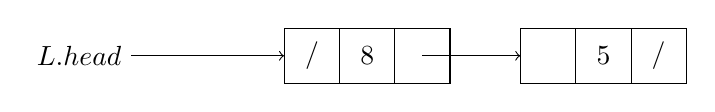
\begin{tikzpicture}
		\draw (3,0) node[minimum size = 0.7cm, draw] (mid4) {8};
		\draw (3.7,0) node[minimum size = 0.7cm, draw] (tail4) {};
		\draw (2.3,0) node[minimum size = 0.7cm, draw] (head4) {/};

		\draw (6,0) node[minimum size = 0.7cm, draw] (mid1) {5};
		\draw (6.7,0) node[minimum size = 0.7cm, draw] (tail1) {/};
		\draw (5.3,0) node[minimum size = 0.7cm, draw] (head1) {};

		\draw (0,0) node [left] (Lhead) {$L.head$};

		\draw [->] (Lhead) -- (head4.west);
		\draw [->] (tail4.center) -- (head1.west);
	\end{tikzpicture}
	\caption*{\textsc{List-Delete}$(L,7)$}
\end{figure}

\begin{figure}[H]
	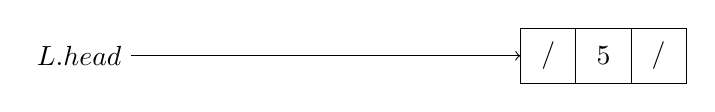
\begin{tikzpicture}
		\draw (6,0) node[minimum size = 0.7cm, draw] (mid1) {5};
		\draw (6.7,0) node[minimum size = 0.7cm, draw] (tail1) {/};
		\draw (5.3,0) node[minimum size = 0.7cm, draw] (head1) {/};

		\draw (0,0) node [left] (Lhead) {$L.head$};

		\draw [->] (Lhead) -- (head1.west);
	\end{tikzpicture}
	\caption*{\textsc{List-Delete}$(L,8)$}
\end{figure}

\section*{Question 8.2}

\begin{figure}[H]
	\begin{minipage}{0.5\textwidth}
		\centering
		\begin{tabular}{ll}
			\toprule
			\multicolumn{2}{l}{$\textsc{Push}S_1(A,x)$} \\
			\midrule
			1. & \textbf{if} $S_2$.top - $S_1$.top == 1 \\
			2. & \quad \textbf{error} ``overflow'' \\
			3. & \textbf{else} \\
			4. & \quad $S_1$.top = $S_1$.top + 1 \\
			5. & \quad $A$[$S_1$.top] = x \\
			\bottomrule
		\end{tabular}
	\end{minipage}
	\begin{minipage}{0.5\textwidth}
		\centering
		\begin{tabular}{ll}
			\toprule
			\multicolumn{2}{l}{$\textsc{Pop}S_1(A)$} \\
			\midrule
			1. & \textbf{if} $S_1$.top == 0 \\
			2. & \quad \textbf{error} ``underflow'' \\
			3. & \textbf{else} \\
			4. & \quad $S_1$.top = $S_1$.top - 1 \\
			5. & \quad \textbf{return} $A$[$S_1$.top + 1] \\
			\bottomrule
		\end{tabular}
	\end{minipage}
	\caption*{Pseudo-code for $S_1$}
\end{figure}

\begin{figure}[H]
	\begin{minipage}{0.5\textwidth}
		\centering
		\begin{tabular}{ll}
			\toprule
			\multicolumn{2}{l}{$\textsc{Push}S_2(A,x)$} \\
			\midrule
			1. & \textbf{if} $S_2$.top - $S_1$.top == 1 \\
			2. & \quad \textbf{error} ``overflow'' \\
			3. & \textbf{else} \\
			4. & \quad $S_2$.top = $S_2$.top - 1 \\
			5. & \quad $A$[$S_2$.top] = x \\
			\bottomrule
		\end{tabular}
	\end{minipage}
	\begin{minipage}{0.5\textwidth}
		\centering
		\begin{tabular}{ll}
			\toprule
			\multicolumn{2}{l}{$\textsc{Pop}S_2(A)$} \\
			\midrule
			1. & \textbf{if} $S_2$.top == $n$ + 1 \\
			2. & \quad \textbf{error} ``underflow'' \\
			3. & \textbf{else} \\
			4. & \quad $S_2$.top = $S_2$.top + 1 \\
			5. & \quad \textbf{return} $A$[$S_2$.top - 1] \\
			\bottomrule
		\end{tabular}
	\end{minipage}
	\caption*{Pseudo-code for $S_2$}
\end{figure}

\section*{Question 8.3}

\begin{center}
	\begin{tabular}{ll}
		\toprule
		\multicolumn{2}{l}{\textsc{Enqueue}$(Q,x)$} \\
		\midrule
		1. & \textbf{if} $Q$.head - $Q$.tail == 1 \textbf{or} ($Q$.head == 1 \textbf{and} $Q$.tail == $Q$.length) \\
		2. & \quad \textbf{error} ``overflow'' \\
		3. & \textbf{else} \\
		4. & \quad $Q$[$Q$.tail] = x \\
		5. & \quad \textbf{if} $Q$.tail == $Q$.length \\
		6. & \quad \quad $Q$.tail = 1 \\
		7. & \quad \textbf{else} \\
		8. & \quad \quad $Q$.tail = $Q$.tail + 1 \\
		\bottomrule
	\end{tabular}
\end{center}

\begin{center}
	\begin{tabular}{ll}
		\toprule
		\multicolumn{2}{l}{\textsc{Dequeue}$(Q)$} \\
		\midrule
		1. & \textbf{if} $Q$.head == $Q$.tail \\
		2. & \quad \textbf{error} ``underflow'' \\
		3. & \textbf{else} \\
		4. & \quad $x$ = $Q$[$Q$.head] \\
		5. & \quad \textbf{if} $Q$.head == $Q$.length \\
		6. & \quad \quad $Q$.head = 1 \\
		7. & \quad \textbf{else} \\
		8. & \quad \quad $Q$.head = $Q$.head + 1 \\
		9. & \quad \textbf{return} $x$ \\
		\bottomrule
	\end{tabular}
\end{center}

\section*{Question 8.4}

\textit{Note: We assume the error handling is done by the stack.}

\textbf{Method 1:}
\begin{center}
	\begin{tabular}{ll}
		\toprule
		\multicolumn{2}{l}{\textsc{Enqueue}$(Q,x)$} \\
		\midrule
		1. & \textbf{while} \textbf{Stack-Empty}$(S_2)$ == FALSE \textbf{do} \\
		2. & \quad \textsc{Push}$(S_1,\textsc{Pop}(S_2))$ \\
		3. & \textsc{Push}$(S_1,x)$ \\
		\bottomrule
	\end{tabular}
\end{center}

\begin{center}
	\begin{tabular}{ll}
		\toprule
		\multicolumn{2}{l}{\textsc{Dequeue}$(Q)$} \\
		\midrule
		1. & \textbf{while} \textbf{Stack-Empty}$(S_1)$ == FALSE \textbf{do} \\
		2. & \quad \textsc{Push}$(S_2,\textsc{Pop}(S_1))$ \\
		3. & \textbf{return} \textsc{Pop}$(S_2)$ \\
		\bottomrule
	\end{tabular}
\end{center}

With this method, the runtime of these two operations depend largely on what is the last operation performed.
If two same operations are performed consecutively, the latter one will be $\Theta(1)$.
If two different operations are performed consecutively, the latter one will be $\Theta(n)$, where $n$ is the number of elements currently in the queue.

\textbf{Method 2:}
\begin{center}
	\begin{tabular}{ll}
		\toprule
		\multicolumn{2}{l}{\textsc{Enqueue}$(Q,x)$} \\
		\midrule
		1. & \textsc{Push}$(S_1,x)$ \\
		\bottomrule
	\end{tabular}
\end{center}

\begin{center}
	\begin{tabular}{ll}
		\toprule
		\multicolumn{2}{l}{\textsc{Dequeue}$(Q)$} \\
		\midrule
		1. & \textbf{if} \textbf{Stack-Empty}$(S_2)$ == TRUE \\
		2. & \quad \textbf{while} \textbf{Stack-Empty}$(S_1)$ == FALSE \textbf{do} \\
		3. & \quad \quad \textsc{Push}$(S_2,\textsc{Pop}(S_1))$ \\
		4. & \textbf{return} \textsc{Pop}$(S_2)$ \\
		\bottomrule
	\end{tabular}
\end{center}

In this method, the runtime of \textsc{Enqueue} is obviously $\Theta(1)$.
The runtime of \textsc{Dequeue} is $\Theta(1)$ in average.

To explain the runtime, for every element in the queue, it will only be pushed into $S_1$ once, popped from $S_1$ once, pushed into $S_2$ once and popped from $S_2$ once.
So the total runtime is $\Theta(4n) = \Theta(n)$.
Since there are $n$ \textsc{Dequeue} operations, the average runtime is $\Theta(1)$.
\end{document}